% \section{Hilft Musik beim lernen?}
% Dieser Frage wollen wir im Folgenden auf den Grund gehen - beziehungsweise versuchen wir es. Ist das überhaupt möglich, die Frage zu beantworten?\\
% Dafür machen wir - was auch sonst - ein kleines Experiment! \\

% Überlege dir eine naturwisenschaftlich sinnvollle (das haben wir ja die letzten Stunden gelernt) Methode, wie man diese Frage beantworten kann.
% Dabei geht es noch nicht darum, dass das Experiment perfekt ist, es geht erst einmal nur darum, dass wir ein paar Ideen sammeln. Notiere dir aber,
% worauf man achten sollte, und welche Probleme es geben könnte. \\


% \writeLines{10}{\textwidth}

\newpage

    \subsection*{Aufgaben mit Musik}
        \subsubsection*{Aufgabe 1}
        Erkläre in ein einem zusammenhängenden Fließtext, wie man vorgehen kann, um zu schauen ob es einen Unterschied macht, welche Form ein Blatt Papier hat, wenn man es fallen lässt. Erkläre zudem dein Ergebnis.

        \begin{flushright}
            
\begin{tikzpicture}
                \node at (0,0){Dauer:};
                \draw(0.75,-0.2)--(3,-0.2);
                \node at (4,0){Sekunden};
            \end{tikzpicture}
        \end{flushright}
    \subsubsection*{Aufgabe 2}
        Berechne folgende Aufgaben im Kopf:

        \begin{align*}
            \randInt{10}{57}+48 & = \\
            455-\randInt{157}{399} & = \\
            3 \cdot \randInt{8}{17} +2 & = \\
            3 \cdot \randInt{21}{48} & = \\
            266 : 14 & = \\
        \end{align*}


        \begin{flushright}
            
\begin{tikzpicture}
                \node at (0,0){Dauer:};
                \draw(0.75,-0.2)--(3,-0.2);
                \node at (4,0){Sekunden};
            \end{tikzpicture}
        \end{flushright}

    \subsubsection*{Aufgabe 3}
        \begin{minipage}[l]{0.6\textwidth}
            Löse die folgende Textaufgabe:
            \begin{itemize}
                \item[a)] Stelle eine Gleichung auf, wie man den Umfang der nebenstehenden Fläche berechnet.
                \item[b)] Wie groß ist der Umfang für den Wert $b=\randInt{1}{6}$ cm?
            \end{itemize}
        \end{minipage}
        \hspace{1.5cm}
        \begin{minipage}[r]{0.35\textwidth}
            \
            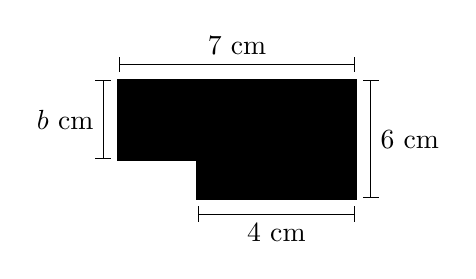
\begin{tikzpicture}
                \filldraw[fill = \mainc, very thick](0,0)--(1,0)--(1,-0.5)--(3,-0.5)--(3,1)--(0,1)--cycle;
                \draw[|-|] (0,1.2)--(3,1.2) node[midway, above]{$7$ cm};
                \draw[|-|] (3.2,1)--(3.2,-0.5) node[midway, right]{$6$ cm};
                \draw[|-|] (3,-0.7)--(1,-0.7) node[midway, below]{$4$ cm};
                \draw[|-|] (-0.2,0)--(-0.2,1) node[midway, left]{$b$ cm};
            \end{tikzpicture}
        \end{minipage}


        \begin{flushright}
            
\begin{tikzpicture}
                \node at (0,0){Dauer:};
                \draw(0.75,-0.2)--(3,-0.2);
                \node at (4,0){Sekunden};
            \end{tikzpicture}
        \end{flushright}

    \newpage
    \subsubsection*{Aufgabe 4}

        \begin{itemize}
            \item[a)] Vereinfache den folgenden Term:

                \begin{align*}
                & \frac{\randInt{1}{15}y}{5}+2+\frac{\randInt{1}{15}}{5}y
                \end{align*}

            \item[b)] Löse die folgende Gleichung nach $x$ auf.
                \begin{align*}
                & 3x-5=25
                \end{align*}
        \end{itemize}


        \begin{flushright}
            
\begin{tikzpicture}
                \node at (0,0){Dauer:};
                \draw(0.75,-0.2)--(3,-0.2);
                \node at (4,0){Sekunden};
            \end{tikzpicture}
        \end{flushright}



    % Gegeben sind folgende Messdaten, zusammen mit einer Ausgleichsgeraden: \\

    % \begin{minipage}{0.49 \textwidth}
    %     \begin{tikzpicture}[>=stealth]
    %         %grid
    %         \draw[help lines, color=gray!30] (0,0) grid (5,5);

    %         \draw[->](0,0)--(5,0) node[right]{$t$ [s]};
    %         \draw[->](0,0)--(0,5) node[left]{$s$ [m]};

    %         \foreach \x in {1,2,3,4}{
    %             \draw (\x,0.1)--(\x,-0.1) node[below]{$\x$};
    %             \draw (0.1,\x)--(-0.1,\x) node[left]{$\x0$};
    %         }

    %         %Messdaten
    %         \fill[orange](1,1.1)circle(0.1);
    %         \fill[orange](1.5,2.5)circle(0.1);
    %         \fill[orange](2,3.1)circle(0.1);
    %         \fill[orange](2.5,3.8)circle(0.1);
    %         \fill[orange](3,4.2)circle(0.1);



    %         \draw[dblue, thick](0,0)--(2,3)--(8/3,4);
    %     \end{tikzpicture}
    % \end{minipage}
    % \begin{minipage}{0.49 \textwidth}
    %     \begin{itemize}
    %         \item[a)] Stelle die Geradengleichung der Ausgleichgeraden auf.
    %         \item[b)] Welche Geschwindigkeit hat der Läufer?
    %         \item[c)] Wie lange benötigt er für 45m?
    %         \item[d)] Wie weit kommt er in 27s?
    %     \end{itemize}
    % \end{minipage}

    \subsubsection*{Aufgabe 5}
    An ihrer Schule besuchen Simon, Claudia, Marius und Ina jeweils eine der vier AGs:\\
    Mathematik, Schach, Chor und Theater. \\
    Von Montag bis Donnerstag findet am Nachmittag jeweils eine der Arbeitsgemeinschaften statt. \\
    Simon und Ina möchten sich verabreden.\\
    Ina schlägt Simon vor: „Können wir uns am Donnerstag mit Marius treffen? Meine AG fällt
    diese Woche ja aus. Ich weiß aber nicht, wann die Mathe-AG, Schach-AG und Theater-AG
    stattfinden.“ \\
    Simon weiß Rat: „Meine Theater-AG ist nicht donnerstags. Mittwochs leitet
    meine Schwester die Schach-AG und dienstags hat Marius seine AG.“\\
    
    Welche Ag besucht Marius?\\
    An welchem Wochentag indet diese statt?


    \begin{flushright}
            
\begin{tikzpicture}
                \node at (0,0){Dauer:};
                \draw(0.75,-0.2)--(3,-0.2);
                \node at (4,0){Sekunden};
            \end{tikzpicture}
        \end{flushright}
    \newpage

\subsection*{Aufgaben ohne Musik}
    \subsubsection*{Aufgabe 1}
        Erkläre in einem zusammenhängenden Fließtext, wie man vorgehen kann, um zu untersuchen, ob man Bliz oder Donner zuerst wahrnimmt. Erkläre zudem dein Ergebnis.


        \begin{flushright}
            
\begin{tikzpicture}
                \node at (0,0){Dauer:};
                \draw(0.75,-0.2)--(3,-0.2);
                \node at (4,0){Sekunden};
            \end{tikzpicture}
        \end{flushright}
    \subsubsection*{Aufgabe 2}
        Berechne folgende Aufgaben im Kopf:

        \begin{align*}
            \randInt{66}{98}+\randInt{22}{45} & = \\
            714-\randInt{218}{613} & = \\
            8/2-5 & = \\
            4 \cdot \randInt{26}{39} & = \\
            216 : 18 & = \\
        \end{align*}


        \begin{flushright}
            
\begin{tikzpicture}
                \node at (0,0){Dauer:};
                \draw(0.75,-0.2)--(3,-0.2);
                \node at (4,0){Sekunden};
            \end{tikzpicture}
        \end{flushright}

\subsubsection*{Aufgabe 3}

    \begin{minipage}[l]{0.6\textwidth}
        Stelle einen Term auf, um den Flächeninhalt der nebenstehenden Form zu berechnen.
    \end{minipage}
    \begin{minipage}[r]{0.35\textwidth}
        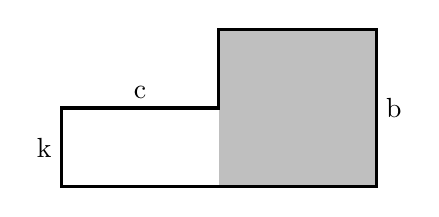
\begin{tikzpicture}
            \fill[lightgray](2,0) rectangle(4,2);
            \draw[very thick](0,0)--(0,1)--(2,1)--(2,2)--(4,2)--(4,0)--cycle;

            \node[right] at (4,1){b};
            \node[left] at (0,0.5){k};
            \node[above] at (1,1){c};
        \end{tikzpicture}
    \end{minipage}


    \begin{flushright}
            
\begin{tikzpicture}
                \node at (0,0){Dauer:};
                \draw(0.75,-0.2)--(3,-0.2);
                \node at (4,0){Sekunden};
            \end{tikzpicture}
        \end{flushright}
    \newpage

\subsubsection*{Aufgabe 4}
    \begin{itemize}
        \item[a)] Klammere eine Zahl mit möglichst großem Betrag aus, sodass alle im Term vorkommenden Zahlen ganze Zahlen bleiben:
        \item[] \begin{align*}
            i)\quad & -36-45w \\
            ii)\quad & 15a-21
            \end{align*}
        \item[b)] Vereinfache die beiden Terme und prüfe, ob sie gleichwertig sind:
        \item[] \begin{align*}
                & \frac{3}{7} \cdot 4z-\left(-9-3z \cdot \frac{3}{7}\right) \\
                \text{und} \quad & 3 \cdot (z-3)
                \end{align*}
    \end{itemize}



    \begin{flushright}
        
\begin{tikzpicture}
            \node at (0,0){Dauer:};
            \draw(0.75,-0.2)--(3,-0.2);
            \node at (4,0){Sekunden};
        \end{tikzpicture}
    \end{flushright}

        % Gegeben sind die folgenden Messdaten:

        % \begin{minipage}{0.49 \textwidth}
        %     \begin{table}[H]
        %         \centering
        %         \begin{tabular}{c|c}  % Spaltenformat: 'c' = zentriert, '|' = vertikale Linie
        %             \hline  % Horizontale Linie oben
        %             $t$ [s] & $v$ [m/s] \\  % Spaltenüberschriften mit mathematischen Variablen
        %             \hline
        %             0 & 0 \\
        %             1 & 2,1 \\  % Dezimalpunkt statt Komma in LaTeX
        %             2 & 3,9 \\
        %             3 & 6,0 \\
        %             4 & 8,2 \\
        %             \hline  % Horizontale Linie unten
        %         \end{tabular}
        %         \caption{Messwerte der Funktion}  % Beschreibung der Tabelle
        %         \label{tab:messwerte}  % Label für Referenzen
        %     \end{table}
        % \end{minipage}
        % \begin{minipage}[c]{0.49 \textwidth}
        %     \begin{itemize}
        %         \item[a)] Stelle die Tabelle graphisch dar.
        %         \item[b)] Stelle eine Funktionsgleichung der Ausgleichsgerade auf.
        %         \item[c)] Welche Geschwindigkeit hat das Objekt nach 8 s?
        %     \end{itemize}
        % \end{minipage}

\subsubsection*{Aufgabe 5}
        Anna, Birgit, Claudia und Daniele besuchen jeweils eine der vier Unis den den Städten  Freiburg, Karlsrhe, Stuttgart und Tübigen. Folgende Informationen sind bekannt:
        \begin{itemize}
            \item Anna und die Tübinger Studentin studieren beide Jura.
            \item Die Stuttgarter Studentin und Birgit studieren beide Mathematik.
            \item Claudia und die Stuttgarter Studentin sind als einzige verheiratet.
            \item Birgit und die Karlsruher Studentin spielen Handball.
        \end{itemize}

        Wo und was studieren die vier Studentinnen?

    \begin{flushright}
            
\begin{tikzpicture}
                \node at (0,0){Dauer:};
                \draw(0.75,-0.2)--(3,-0.2);
                \node at (4,0){Sekunden};
            \end{tikzpicture}
        \end{flushright}







% \subsection{Worum ging es?}
% Um etwas in die Welt der Naturwissenschaft einzutauchen haben wir in den
% letzten Stunden einige kleine Experimente durchgeführt, und zum Teil auch vollständig ausgewertet und diskutiert.\\
% Notiere dir hier, was wir in unseren Experimenten, die wir gemacht haben, rausfinden wollten. \\

% \writeLines{8}{\textwidth}

% \newpage

% \subsection{Wie sah das Experiment aus?}

% Beschreibe hier, was wir für ei Experiment gemacht haben, um herauszufinden, was wir rausfinden wollten.\\
% Warum war das geeignet? Du kannst gerne Skizzen benutzen (das ist sowieso immer sinnvoll ;-) \\

% \karoBox{\textwidth}{10cm}

% \newpage

% \subsection{Auswertung des Experimentes}

% Beschreibe nun, wie wir nun durch das Experiment unsere Anfangsfrage beantworten konnten.\\

% \karoBox{\textwidth}{9cm}

% \subsection{Was ist Naturwissenschaft?}

% Kannst du nun nocheinmal für dich auschreiben/definieren, was Naturwissenschaft ist, und wodurch sie sich auszeichnet? \\

% \drawbox{\textwidth}{3cm}